%---------- Inleiding ---------------------------------------------------------

\section{Introductie}%
\label{sec:introductie}

%Waarover zal je bachelorproef gaan? Introduceer het thema en zorg dat volgende zaken zeker duidelijk aanwezig zijn:

%\begin{itemize}
%  \item kaderen thema
%  \item de doelgroep
%  \item de probleemstelling en (centrale) onderzoeksvraag
%  \item de onderzoeksdoelstelling
%\end{itemize}

%Denk er aan: een typische bachelorproef is \textit{toegepast onderzoek}, wat betekent dat je start vanuit een concrete probleemsituatie in bedrijfscontext, een \textbf{casus}. Het is belangrijk om je onderwerp goed af te bakenen: je gaat voor die \textit{ene specifieke probleemsituatie} op zoek naar een goede oplossing, op basis van de huidige kennis in het vakgebied.

%De doelgroep moet ook concreet en duidelijk zijn, dus geen algemene of vaag gedefinieerde groepen zoals \emph{bedrijven}, \emph{developers}, \emph{Vlamingen}, enz. Je richt je in elk geval op it-professionals, een bachelorproef is geen populariserende tekst. Eén specifiek bedrijf (die te maken hebben met een concrete probleemsituatie) is dus beter dan \emph{bedrijven} in het algemeen.

%Formuleer duidelijk de onderzoeksvraag! De begeleiders lezen nog steeds te veel voorstellen waarin we geen onderzoeksvraag terugvinden.

%Schrijf ook iets over de doelstelling. Wat zie je als het concrete eindresultaat van je onderzoek, naast de uitgeschreven scriptie? Is het een proof-of-concept, een rapport met aanbevelingen, \ldots Met welk eindresultaat kan je je bachelorproef als een succes beschouwen?


In onze huidige maatschappij wordt in bijna elke job gebruikgemaakt van digitale technologieën. Vooral na de COVID-19-pandemie nam het belang van computervaardigheden toe, doordat meer werknemers op afstand gingen werken \autocite{NBERw27422}. Zoals blijkt uit gegevens van de Federale Overheidsdienst Economie, beschikken individuen met een lager opleidingsniveau, lager inkomen of hogere leeftijd vaak niet over de nodige computervaardigheden waardoor ze digitaal uitgesloten worden \autocite{FederalPublicServiceEconomyKloof}.

Daarom, in lijn met de 'Digital Decade' visie van de Belgische overheid, die streeft naar een digitaal competente samenleving tegen 2030 \autocite{DigitalDecade2030}, richt dit onderzoeksvoorstel zich op het verminderen van de digitale kloof op de werkvloer. Het doel is om zowel sollicitanten als huidige werknemers met een beperkte ICT-kennis (bijvoorbeeld arbeiders, magazijniers, logistiek medewerkers) te testen op hun computervaardigheden zodat zij zich, indien gewenst, kunnen bijscholen.

Centraal in dit onderzoek staat de vraag: 'Hoe kan een webapplicatie de computervaardigheden van deze werknemers beoordelen en bijdragen aan het verminderen van digitale uitsluiting?'. Om deze digitale kloof te overbruggen is er behoefte aan een webtool om de computervaardigheden van personen te kunnen beoordelen.
Deze tool geeft aan welke computervaardigheden sollicitanten het best kunnen verbeteren en helpt werkgevers bij het beoordelen van sollicitanten. Het doel van de webtool is de digitale kloof op de werkvloer te verkleinen.

Het uiteindelijke resultaat van deze studie is een proof-of-concept voor een webapplicatie, wa\-arbij de gebruiker een score ontvangt gebaseerd op correctheid, tijd en het aantal hints bij elke vraag. Deze scores geven inzicht in de huidige digitale vaardigheden en dienen bovendien ook als leidraad voor gerichte training en ontwikkeling, met als doel het verkleinen van de digitale kloof.

De kern van dit onderzoek richt zich op het ontwerpen en ontwikkelen van computervaardigheidstesten, waarbij de focus ligt op het correct opstellen van de testen en het berekenen van de resultaten. Voor deze doeleinden wordt gebruik gemaakt van een eenvoudige website en virtualisatietechnieken. Dit houdt in dat, hoewel het project technische aspecten zoals webontwikkeling en virtualisatie bevat, de nadruk voornamelijk ligt op de ontwikkeling van de testen zelf en op de communicatie tussen de testomgeving en de website.

%---------- Stand van zaken ---------------------------------------------------

\section{Literatuurstudie}%
\label{sec:state-of-the-art}

%Hier beschrijf je de \emph{state-of-the-art} rondom je gekozen onderzoeksdomein, d.w.z.\ een inleidende, doorlopende tekst over het onderzoeksdomein van je bachelorproef. Je steunt daarbij heel sterk op de professionele \emph{vakliteratuur}, en niet zozeer op populariserende teksten voor een breed publiek. Wat is de huidige stand van zaken in dit domein, en wat zijn nog eventuele open vragen (die misschien de aanleiding waren tot je onderzoeksvraag!)?

%Je mag de titel van deze sectie ook aanpassen (literatuurstudie, stand van zaken, enz.). Zijn er al gelijkaardige onderzoeken gevoerd? Wat concluderen ze? Wat is het verschil met jouw onderzoek?

%Verwijs bij elke introductie van een term of bewering over het domein naar de vakliteratuur, bijvoorbeeld\autocite{Hykes2013}! Denk zeker goed na welke werken je refereert en waarom.

%Draag zorg voor correcte literatuurverwijzingen! Een bronvermelding hoort thuis \emph{binnen} de zin waar je je op die bron baseert, dus niet er buiten! Maak meteen een verwijzing als je gebruik maakt van een bron. Doe dit dus \emph{niet} aan het einde van een lange paragraaf. Baseer nooit teveel aansluitende tekst op eenzelfde bron.

%Als je informatie over bronnen verzamelt in JabRef, zorg er dan voor dat alle nodige info aanwezig is om de bron terug te vinden (zoals uitvoerig besproken in de lessen Research Methods).

% Voor literatuurverwijzingen zijn er twee belangrijke commando's:
% \autocite{KEY} => (Auteur, jaartal) Gebruik dit als de naam van de auteur
%   geen onderdeel is van de zin.
% \textcite{KEY} => Auteur (jaartal)  Gebruik dit als de auteursnaam wel een
%   functie heeft in de zin (bv. ``Uit onderzoek door Doll & Hill (1954) bleek
%   ...'')

%Je mag deze sectie nog verder onderverdelen in subsecties als dit de structuur van de tekst kan verduidelijken.
%PROBLEEMSTELLING
\subsection{Digitale Kloof en haar Impact}
Uit een onderzoek van de \textcite{VlaamseVeerkracht} naar de digitale vaardigheden bij burgers blijkt dat 46\% van de Vlaamse bevolking tussen 16 en 74 jaar niet beschikt over de nodige digitale basisvaardigheden: 37\% heeft lage digitale vaardigheden en 8\% heeft geen digitale vaardigheden of heeft in de voorbije 3 maanden geen internet gebruikt.
Bovendien bevestigt \textcite{DigitaleInclusieBarometer} in een onderzoek over de digitale inclusie van de Koning Boudewijnstichting dat een groot deel van de Belgen kwetsbaar zijn voor uitsluiting van essentiële diensten zoals werk, onderwijs en gezondheidszorg omdat zij over onvoldoende digitale vaardigheden beschikken.

De digitale ongelijkheid is een realiteit. \textcite{IedereenDigitaleKloof} van het Vlaams Steunpunt Nieuwe Geletterdheid merkt in een artikel op dat de digitale kloof geen ééndimensioneel probleem is. Naast het bezit van computers en de instrumentele vaardigheden bestaat de digitale kloof immers uit nog andere facetten. Zo heeft men tevens informatievaardigheden nodig. Dit zijn methodes om online informatie op te sporen: zoeken, selecteren, begrijpen, evalueren en verwerken. Maar zelfs tot het toepassen van digitale informatievaardigheden op een eenvoudig niveau, namelijk het gebruiken van een zoekmachine, is 1/3 van de Belgische bevolking niet in staat.
Daarbij heeft de coronapandemie de digitalisering van de maatschappij aanzienlijk versneld. Zoals aangegeven door \textcite{VlaamseVeerkracht} ging het digitaliseringsproces de afgelopen jaren gepaard met het geleidelijk verdwijnen van een aantal fysieke loketten. Daar konden nochtans vele burgers terecht en werden ze geholpen als ze administratieve problemen hadden. Deze toegenomen digitalisering heeft gevolgen op veel maatschappelijke domeinen zoals bankdiensten, mobiliteit, gezondheidszorg en onderwijs.

%\subsection{Belang van Computervaardigheden}
Dit onderzoeksvoorstel richt zich op de digitalisering in de werkomgeving, met speciale aandacht voor sollicitanten en huidige werknemers met beperkte ICT-kennis zoals arbeiders, magazijniers en logistiek medewerkers. Het doel is om hun computervaardigheden te testen en hen de mogelijkheid te bieden zich bij te scholen, in lijn met het doel van de Vlaamse overheid om minstens 80\% van de bevolking digitaal vaardig te maken.
Deze studie focust op het testen van essentiële digitale vaardigheden zoals gedefinieerd in het DigComp-raamwerk van het Joint Research Centre van de Europese Commissie. Deze omvatten het opzoeken en verwerken van informatie, het maken van PDF-documenten, het vinden van bestanden op de computer, e-mailen en het uploaden van bestanden \autocite{DigCompFramework}. Deze vaardigheden zijn cruciaal voor een effectieve digitale communicatie en organisatie in de moderne werkomgeving.

\subsection{Beoordeling computervaardigheden}
Om de computervaardigheden van individuen op een betrouwbare en nauwkeurige manier te beoordelen, is het ontwikkelen van een webapplicatie met concrete ICT-opdrachten gepland. Traditionele vragenlijsten, zoals die op de website van de VDAB, zijn voornamelijk theoretisch van aard en geven geen nauwkeurig beeld van de praktische vaardigheden.
De geplande webapplicatie zal in tegenstelling tot deze traditionele methoden praktijkgerichte oefeningen bevatten. Dit is in overeenstemming met bevindingen uit onderzoek dat aangeeft dat het onderhouden van georganiseerde informatierepositories bijdraagt aan een groter vertrouwen in eigen kennis \autocite{JudgingKnowledge}.
Daarnaast onderstrepen de DESI-rapporten 2021 en 2022 de noodzaak van dit onderzoek. Het DESI 2022-rapport benadrukt dat, hoewel België aanzienlijke vooruitgang heeft geboekt op het gebied van digitale connectiviteit en de integratie van digitale technologieën in bedrijven, er nog steeds aanzienlijke ruimte is voor verbetering in digitale vaardigheden \autocite{DESIRaport}. Deze  informatie ondersteunt de relevantie van het onderzoeksvoorstel binnen het bredere maatschappelijke en economische kader van België.
Ten slotte biedt het DigComp-raamwerk van het Joint Research Centre van de Europese Commissie een nuttig referentiekader voor het definiëren van digitale competenties en vaardigheden, wat relevant kan zijn voor de ontwikkeling van de webapplicatie \autocite{DigCompFramework}.

%SOFTWARE
%uitleggen website
\subsection{Rol van webapplicaties in vaardigheidstesten}
Bovenvermelde informatie rechtvaardigt de k\-euze voor een webapplicatie. Gebruikers met onvoldoende basiskennis van ICT slagen er vaak niet in om software correct te installeren. Het gebruik van een webapplicatie maakt het mogelijk om de testen in een veilige virtuele omgeving uit te voeren zodat de gebruiker geen schade kan aanbrengen aan zijn eigen digitale omgeving. De webapplicatie zal dus fungeren als een communicatiemiddel tussen de Windows-omgeving, waar de testen zullen worden uitgevoerd, en de gebruiker.

%uitleggen OS
De keuze voor een Windows-omgeving om computervaardigheidstesten uit te voeren, is ingegeven door de brede verspreiding en populariteit van Windows als besturingssysteem. Volgens een rapport van \textcite{StatCounterOSMarketShare} heeft Windows een aanzienlijk marktaandeel in desktopbesturingssystemen in België, wat aangeeft dat het algemeen bekend en geaccepteerd is in de professionele wereld. Dit wordt verder ondersteund door het feit dat Windows vaak het standaard besturingssysteem is bij de aanschaf van nieuwe computers \autocite{ProfolusWindowsPopularity}.

%uitleggen VM
\subsection{Gebruik van virtualisatietechnologieën}
De Windows-omgevingen kunnen worden opgezet via virtualisatie. 'Met virtualisatie wordt een gesimuleerde, oftewel virtuele, computeromgeving gemaakt, dit in tegenstelling tot een fysieke omgeving. Bij virtualisatie gaat het vaak om door een computer gegenereerde versies van hardware, besturingssystemen, opslagapparaten en meer.' \autocite{MicrosoftVirtualisationDefinition}.

Een virtualisatiesoftwarepakket, zoals VirtualBox, wordt gebruikt om virtuele machines te creëren en te beheren op een fysieke computer of server. Dit maakt het mogelijk om meerdere virtuele Windows-omgevingen te maken, elk met de vereiste applicatie voor het beoordelen van testen. De keuze voor VirtualBox is gebaseerd op verschillende factoren, waaronder het feit dat het een populaire en open source virtualisatiesoftware is. Verder biedt VirtualBox handige functies zoals het maken van snapshots, waardoor het beheer van virtuele machines efficiënter wordt en het gebruik van bronnen wordt geoptimaliseerd. VBoxManage is een command-line tool waarmee VirtualBox volledig bestuurd kan worden.

%uitleggen connectie VM met website
\subsection{Interactie met testomgeving}
Om interactie mogelijk te maken met een Wi\-ndows-omgeving en deze te integreren in een webapplicatie, is een tool nodig die verbinding kan maken met deze Windows-omgeving. Apache Guacamole is een uiterst geschikt framework dat ondersteuning biedt voor een breed scala aan protocollen, waaronder VNC, RDP, SSH en meer. Hierdoor kun je verschillende soorten externe verbindingen beheren en naadloos schakelen tussen diverse systemen zonder de noodzaak van aparte tools.
Met Apache Guacamole kan een beveiligde verbinding worden gemaakt met de virtuele Windows-omgeving. Dit stelt de gebruiker in staat om veilig en efficiënt te werken in de Windows-omgeving via de webapplicatie. \autocite{ApacheGuacamole}.

%uitleggen API
\subsection{API's en systeemintegratie}
Het is noodzakelijk om communicatie tussen de testen op de virtuele machine en de webapplicatie mogelijk te maken. Hiervoor wordt een Application Programming Interface (API) ontwikkeld. 'Een API biedt een eenvoudige manier om verbinding te maken met softwaresystemen en deze te integreren en uit te breiden.' \autocite{biehl2015api}. De noodzaak van een API in dit onderzoeksproject ontstaat uit de beperkingen van de webapplicatie om direct te interageren met de Windows-omgevingen, waar de computervaardigheidstests worden uitgevoerd. De API speelt een cruciale rol bij het opslaan van testresultaten en het beschikbaar stellen ervan aan de webapplicatie. Bovendien zal de API gebruikt worden om de virtuele machines op afstand te beheren en te starten.


%---------- Methodologie ------------------------------------------------------
\section{Methodologie}%
\label{sec:methodologie}

%Hier beschrijf je hoe je van plan bent het onderzoek te voeren. Welke onderzoekstechniek ga je toepassen om elk van je onderzoeksvragen te beantwoorden? Gebruik je hiervoor literatuurstudie, interviews met belanghebbenden (bv.voor requirements-analyse), experimenten, simulaties, vergelijkende studie, risico-analyse, PoC, \ldots?

%Valt je onderwerp onder één van de typische soorten bachelorproeven die besproken zijn in de lessen Research Methods (bv.\ vergelijkende studie of risico-analyse)? Zorg er dan ook voor dat we duidelijk de verschillende stappen terug vinden die we verwachten in dit soort onderzoek!

%Vermijd onderzoekstechnieken die geen objectieve, meetbare resultaten kunnen opleveren. Enquêtes, bijvoorbeeld, zijn voor een bachelorproef informatica meestal \textbf{niet geschikt}. De antwoorden zijn eerder meningen dan feiten en in de praktijk blijkt het ook bijzonder moeilijk om voldoende respondenten te vinden. Studenten die een enquête willen voeren, hebben meestal ook geen goede definitie van de populatie, waardoor ook niet kan aangetoond worden dat eventuele resultaten representatief zijn.

%Uit dit onderdeel moet duidelijk naar voor komen dat je bachelorproef ook technisch voldoen\-de diepgang zal bevatten. Het zou niet kloppen als een bachelorproef informatica ook door bv.\ een student marketing zou kunnen uitgevoerd worden.

%Je beschrijft ook al welke tools (hardware, software, diensten, \ldots) je denkt hiervoor te gebruiken of te ontwikkelen.

%Probeer ook een tijdschatting te maken. Hoe lang zal je met elke fase van je onderzoek bezig zijn en wat zijn de concrete \emph{deliverables} in elke fase?

In de initiële fase van het project, die twee weken duurt, wordt een requirements-analyse uitgevoerd. De focus ligt hierbij op het identificeren van relevante digitale testen die ontwikkeld kunnen worden.
Daarnaast worden de technische en functionele vereisten voor de API, de webapplicatie en de virtuele Windows-omgeving gedetailleerd vastgesteld. Ten slotte omvat deze fase het ontwikkelen van een intuïtief en gebruikersvriendelijk ontwerp voor de UI/UX van de webapplicatie.

De volgende fase van het project heeft een duur van 3 weken. In deze periode wordt een API ontworpen. Deze API is bedoeld voor het beheren en opstarten van virtuele machines met VBoxManage. Daarnaast zal de API testresultaten opslaan en deze toegankelijk maken voor de webapplicatie. Een belangrijke functionaliteit van de API is ook het vermogen om virtuele machines op afstand te starten.

In de derde fase, die ook twee weken duurt, wordt de website opgezet om verbinding te maken met de virtuele omgeving. Deze wordt geconfigureerd met Apache Guacamole, waardoor gebruikers, zodra zij een test starten op de webapplicatie, kunnen interacteren met de Windows-omgeving.

De vierde fase neemt 4 weken in beslag. Hierbij worden de vaardigheidstesten ontwikkeld waarvan de data na afloop doorgestuurd wordt naar de API. Er wordt een applicatie ontwikkeld die in de Windows-omgeving zal runnen. De applicatie zal samen met de virtuele Windows-omgeving opstarten. Deze zal een scenario aan de gebruiker geven waarin hij enkele realistische taken moet uitvoeren. Deze applicatie zal de gemaakte taken controleren en een resultaat toekennen.

In de vijfde fase van het project, die 2 weken zal duren, worden de testresultaten vanuit de API opgehaald en in de webapplicatie weergegeven. De testen zijn opgesteld met als doel de gebruiker te helpen bij het ontwikkelen en verbeteren van zijn computervaardigheden.

Tot slot wordt in de laatste fase van het project, die twee weken duurt, een scriptie opgesteld. Hierin worden het volledige onderzoek en de behaalde resultaten gedetailleerd beschreven. De scriptie vormt een uitgebreid verslag van het uitgevoerde onderzoek, inclusief een beschrijving van de gebruikte methodologie en de uitgevoerde werkzaamheden. Het biedt een overzicht van de genomen stappen tijdens het onderzoek.


\begin{figure}[ht]
  \centering
  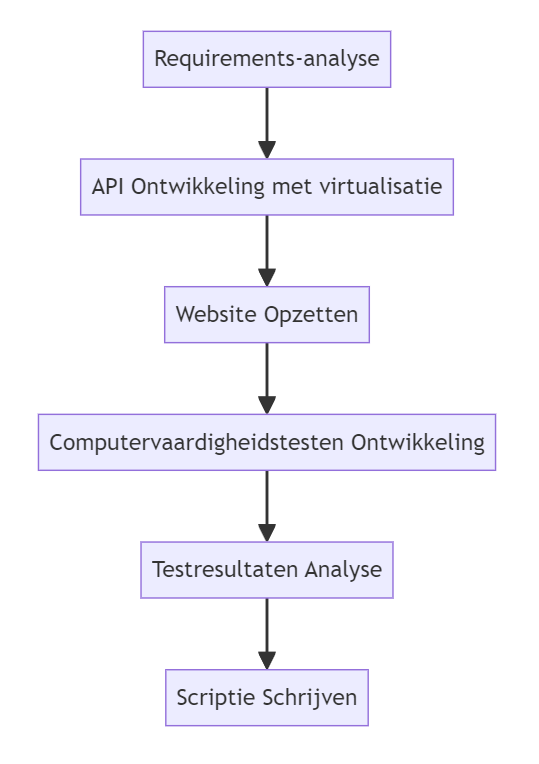
\includegraphics[width=\linewidth]{./graphics/flowchart.png}
  \caption{Flowchart}
  \label{fig:flowchart}
\end{figure}

\begin{figure}[ht]
  \centering
  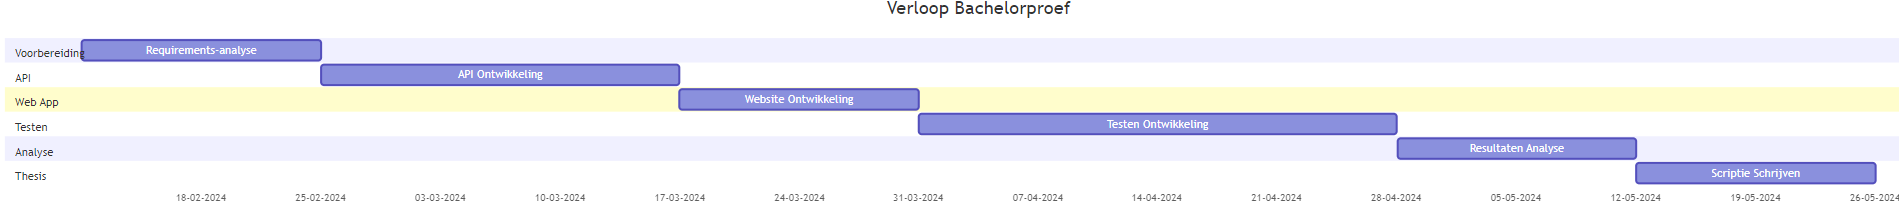
\includegraphics[width=\linewidth]{./graphics/gantt.png}
  \caption{Gantt Diagram}
  \label{fig:gantt}
\end{figure}

%Dit geautomatiseerde proces bespaart tijd voor de werkgever en de sollicitant.

%Na het verkrijgen van de testresultaten kan de werkgever de sollicitant of huidige werknemer cursussen aanbieden om zijn computervaardigheden bij te schaven. Op die manier zijn werknemers up-to-date met bedrijfsspecfieke software en beschikken ze over basis ICT-kennis. Dit kan een eerste stap zijn naar het verkleinen van de digitale kloof.

%---------- Verwachte resultaten ----------------------------------------------
\section{Verwacht resultaat, conclusie}%
\label{sec:verwachte_resultaten}

%Hier beschrijf je welke resultaten je verwacht. Als je metingen en simulaties uitvoert, kan je hier al mock-ups maken van de grafieken samen met de verwachte conclusies. Benoem zeker al je assen en de onderdelen van de grafiek die je gaat gebruiken. Dit zorgt ervoor dat je concreet weet welk soort data je moet verzamelen en hoe je die moet meten.

%Wat heeft de doelgroep van je onderzoek aan het resultaat? Op welke manier zorgt jouw bachelorproef voor een meerwaarde?

%Hier beschrijf je wat je verwacht uit je onderzoek, met de motivatie waarom. Het is \textbf{niet} erg indien uit je onderzoek andere resultaten en conclusies vloeien dan dat je hier beschrijft: het is dan juist interessant om te onderzoeken waarom jouw hypothesen niet overeenkomen met de resultaten.

De uitvoering van dit project zal resulteren in een webapplicatie die zowel gebruikers als werkgevers voorziet van nauwkeurige inzichten in computervaardigheden. Gebruikers krijgen een  overzicht van hun sterke en zwakke punten, terwijl werkgevers het ICT-kennisniveau van sollicitanten en werknemers kunnen beoordelen. Afhankelijk van de testresultaten, kunnen werkgevers gerichte bijscholingsmogelijkheden aanbieden. Uiteindelijk zal deze tool bijdragen aan het verkleinen van de digitale kloof in het bedrijfsleven door het bieden van een praktische oplossing voor het identificeren en aanpakken van tekorten in digitale vaardigheden.